\chapter{Data Analysis}
\label{Chapter:DataAnalysis}
In this chapter we will present how the simulation is run and how the results are analyzed.

\section{Running the simulation}
In order to run a simulation three things are needed:

\begin{itemize}
    \item \textbf{simulation software:} Which is a binary file of the simulation software available for Mac/Win/Linux
    \item \textbf{Simulation Parameters:} A JSON text file that defines simulation parameters
    \item \textbf{Classroom Profile:} A JSON text file that specifies the psychological profiles of students in the class
\end{itemize}

The simulation can be run interactively making it possible to observe the progression
of the simulation, or in headless mode, where no visualization is generated.
The later one is particularly useful when combined with a increased simulation
speed, in which case many different simulations can be run in a \textbf{batch mode}
\footnote{Batch mode means that a series of simulations are run consecutively without
any human supervision or interaction.} like manner.

\bb

Independent of the way the simulation is run, a CSV output file will be generated that
documents the progress of the simulation. That CSV file can be opened in any
arbitrary tabular data processing software (e.g Excel) for manual inspection, but
is made to be analyzed by a set of python scripts developed for the purpose, and
included with the simulation software stack.

How those scripts are used and what results they generate is described in the following chapter.

\section{Data Analysis Pipeline}
The Data Analysis performed for the complete thesis is split into three parts, each 
having a distinct focus, answering a different set of questions.

\begin{enumerate}
    \item \textbf{Simulation:} The goal of the simulation is to study the behavior
    of a particular classroom and combination of agent profiles. Providing insights
    into the behavior of a single agent and the aggregated and averaged behavior of
    the group as a whole.
    \item \textbf{Experiment:} The \textit{Experiment} studies how much variation
    is there between multiple runs of the simulation of the same classroom,
    slightly changing the classroom profiles and random elements of the simulation.
    \item \textbf{Study:} Having a expectation on how a specific classroom profile
    behaves, the \textit{Study} phase asks the question how two different profiles
    compare to each other, and how alterations of the personality profile affect
    group averages.
\end{enumerate}

In the following sections we will have a look at each step of the pipeline individually,
as it is not necessary to run the complete pipeline but based on the question
one tries to answer only one or two of the first steps are necessary.

%%%%%%%%%%%%%%%%%%%%%%%%%%%%%%%%%%%%%%%%%%%%%%%%%%%%%%%%%%%%%%%%%%%%%%%%%%%%%%%%

\section{Simulation}
\textit{Simulation} is the first step of the analysis, answering the question how
a specific classroom of agents behaves.

\begin{figure}[H]
   \hspace*{-4.0\leftmargin}
    \makebox[\textwidth][c]{%
    \begin{minipage}[t]{12cm}
        \centering
        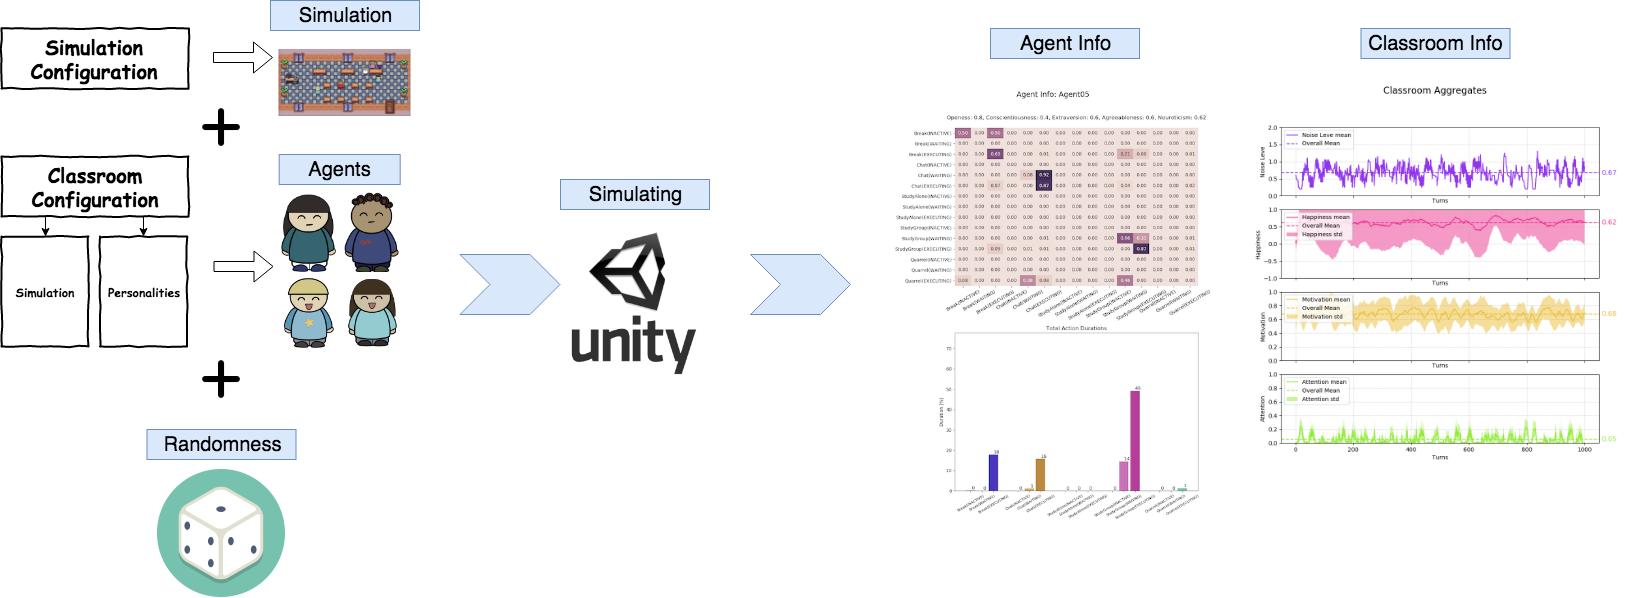
\includegraphics[width=550pt]{Simulation-Overview}
    \end{minipage}    
    }%
    \caption{Simulation Overview}
    \label{SimulationOverview}
\end{figure}

The simulation program takes three input arguments. The simulation config,
is defining all simulation relevant parameters that govern how the simulation mechanism
works, the classroom configuration that defines the psychological profile of students,
and a random seed that is used to initialize the random number generator used during
the simulation.

Examples files of the simulation config and classroom config can be found as part of
the appendix (see \ref{ApxSimulationConfig} and \ref{ApxClassroomProfile}).

The classroom configuration must contain a set of Personality Types and the number
of students of each type. When the simulation is run, a classroom is dynamically
generated and filled with agents as defined.

The python analysis scripts for the simulation will process the CSV file produced
after the simulation is completed and will generate a set of figures containing information
about each individual agent, the classroom as a group and a new CSV file that contains
aggregated information.

\subsection{Agent Info}
One of the results of the simulation step is the \textbf{Agent Info} figure
(see \ref{AgentInfo}) that is generated for each agent, and contains information
about the distribution and transitions between different behaviors performed by the agent.
This figure is used to study how a specific instance of a psychological type behaves
in the given classroom. One can observe how much of the overall time an Agent
spends Studying alone or how long on average a single study session lasts.

\begin{figure}[H]
    \centering
    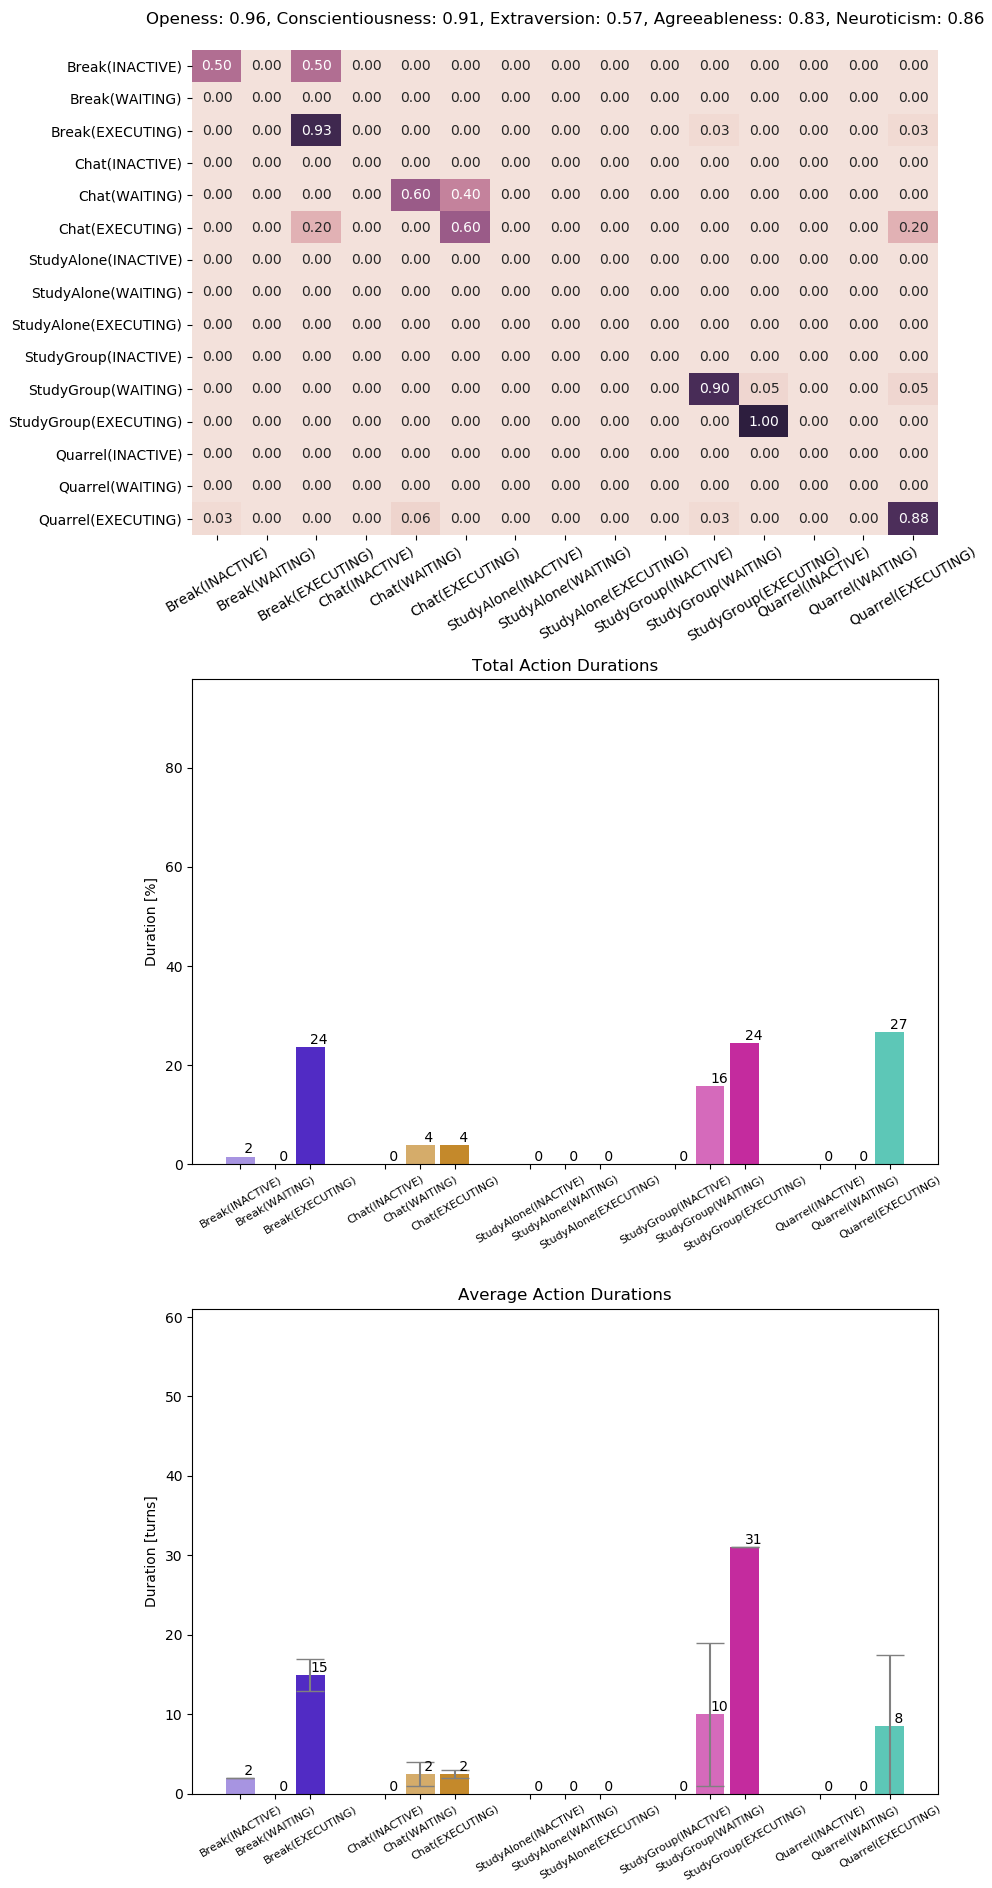
\includegraphics[width=300pt]{AgentInfo1}
    \caption{Agent Info}
    \label{AgentInfo}
\end{figure}

It is interesting to observe the different patterns with which the personality traits
affect the behavior distribution of the individual agents. One could for example
observe that agents higher on conscientiousness, on average have longer
learning sessions.

\subsection{Classroom Aggregates}
The second result produced by the simulation analysis is a figure showing classroom
aggregated features over time (see figure \ref{ClassroomAggregates} as an example).
This figures contains information like the aggregated noise, average happiness,
motivation and attention of a class, in addition to information about how many of
the students are studying or quarreling at a specific moment during the simulation.

This kind of figure is useful to study how personality profiles effect the group
as a whole, and can be used to search for emerging social phenomena.

\begin{figure}[]
    \hspace*{-1.0\leftmargin}
    \makebox[\paperwidth][l]{%
    \begin{minipage}[t]{10cm}
        \centering
        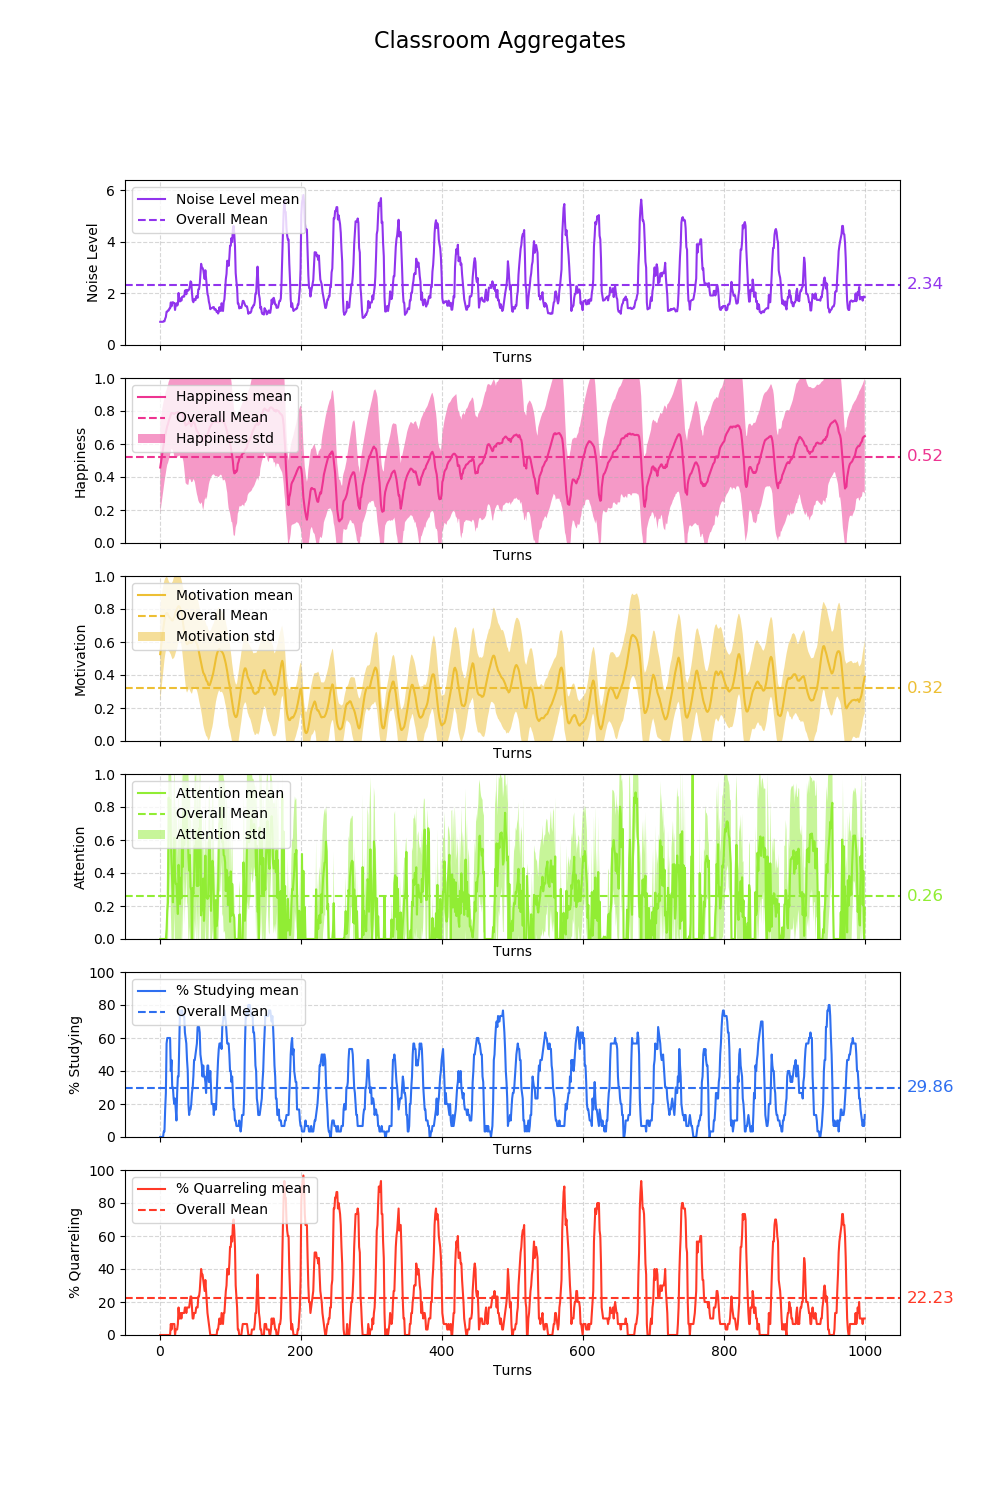
\includegraphics[width=450pt]{ClassroomAggregates}
    \end{minipage}    
    }%
    \caption{Classroom Aggregates}
    \label{ClassroomAggregates}
\end{figure}


%%%%%%%%%%%%%%%%%%%%%%%%%%%%%%%%%%%%%%%%%%%%%%%%%%%%%%%%%%%%%%%%%%%%%%%%%%%%%%%%

\section{Experiment}
The experiment is the second phase of the data analysis pipeline and is focused
on evaluating the variance between simulations of the same classroom configuration.

\begin{figure}[H]
    \makebox[\textwidth][l]{%
    \begin{minipage}[t]{10cm}
        \centering
        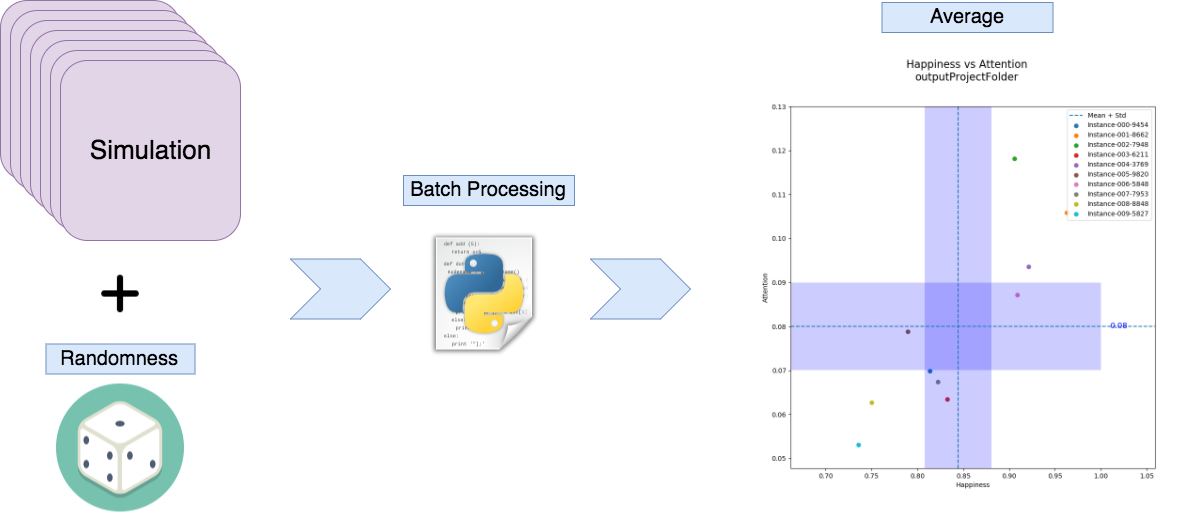
\includegraphics[width=400pt]{Experiment-Overview}
    \end{minipage}    
    }%
    \caption{Experiment Overview}
    \label{ExperimentOverview}
\end{figure}

In order to have a statistical description of the simulation results, one has to
run multiple instances of the same simulation (identical simulation  and classroom
configs) but different seed values for the random number generator used during the simulation.

There are several random elements in the simulation. Depending on the classroom
configuration, agent personality can be partially randomized. The actions selection
process has a random element, and agent interactions are effected by the output of
a random number generator.

\bb

The result of the experiment phase is a single \textbf{HA-Plot}, named after
its axis Attention and Happiness. The plot shows a single point for each simulation
instance, with its position being based on the average attention and happiness of
the corresponding classroom over the complete simulation.

In addition the average happiness and attention over all instances is
indicated with two solid lines, and the corresponding standard deviation with
semi transparent bars.

The plot helps to identify the spread between different instances of the simulation, and
could be used to detect outliers and estimate the stability of a specific classroom
configuration.

In addition to the HA-Plot a CSV file is generated that contains the average
happiness and attention for each agent and classroom for all simulation instances.
This dataset is the numeric equivalent to the generated HA-Plot.

%%%%%%%%%%%%%%%%%%%%%%%%%%%%%%%%%%%%%%%%%%%%%%%%%%%%%%%%%%%%%%%%%%%%%%%%%%%%%%%%

\section{Study}

\begin{figure}[H]
    \makebox[\textwidth][l]{%
    \begin{minipage}[t]{10cm}
        \centering
        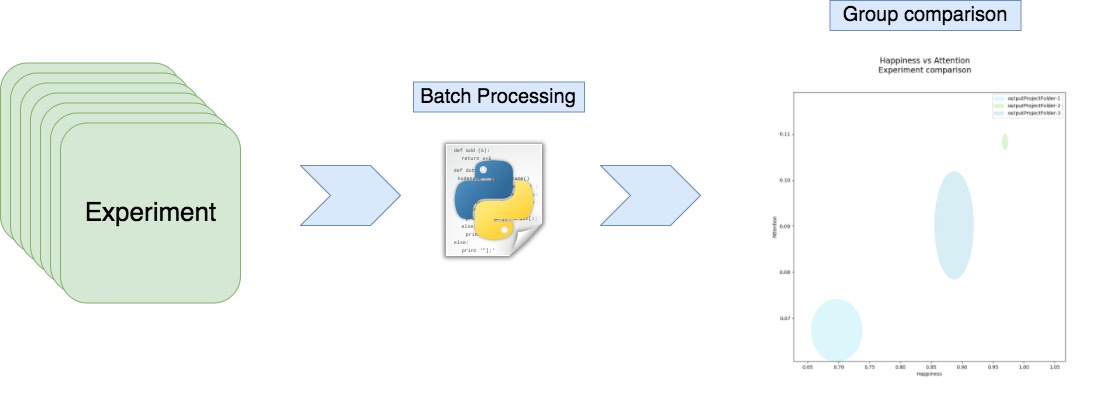
\includegraphics[width=400pt]{Study-Overview}
    \end{minipage}    
    }%
    \caption{Study Overview}
    \label{StudyOverview}
\end{figure}


The last step in the data analysis pipeline is focused on comparing different classroom
profiles.

In this phase of the analysis the CSV generated during the Experiment phase is analyzed to
generate a HA-Plot that contains one ellipse for each classroom profile simulated.
The ellipse center and size are defined by the mean and standard deviation of all
individual agents of the corresponding classroom profile.

This plot gives a visual overview of how the different classroom profiles
compare to each other, and can be used to study the strength and direction of
change one profile has compared to another.

In addition the plot contains a statistical analysis of the relation between
classroom profiles and the correlation between happiness, attention and the different
personality dimensions.

The statistical analysis includes a MANOVA analysis indicating if there is a
significance difference between groups along the dimensions Happiness and Attention,
in addition to a pair wise ANOVA analysis to indicate if each classroom profile
pair is significantly different to each other.

An example of the plot can been seen as part of the results presented in the next
chapter (see figure \ref{StudyResults}).
